\documentclass{acm_proc_article-sp}

% UTF8 encoding and scalable fonts
\usepackage[utf8]{inputenc}
\usepackage[T1]{fontenc}

\usepackage{microtype}
\usepackage{graphicx}
\usepackage{subfigure}
\usepackage{booktabs}
\usepackage{listings}
\usepackage[hyphens]{url}
\usepackage[hidelinks]{hyperref}

% \usepackage{doi}
% \setlength{\paperheight}{11.69in}

\begin{document}

% Leave as is
\conferenceinfo{6th Seminar on Research Trends in Media Informatics (RTMI '14).}{\\February 2014, Ulm University, Ulm, Germany.}
\CopyrightYear{2014}

\title{Interaction Issues during Autonomous Driving}

\numberofauthors{1}
\author{
\alignauthor
Tamino P.S.M. Hartmann\\
       \affaddr{Institute of Media Informatics}\\
       \affaddr{Ulm University}\\
       \affaddr{Ulm, Germany}\\
       \email{tamino.hartmann@uni-ulm.de}
}

% Hyphenations here:
\hyphenation{au-ton-o-mous}

%TODO Citations are missing in section 2.2.2 (i.e. moving the car from stillstand isn't allowed), 2.2.3 (i.e. ...one journalist...) and so on

\maketitle
\begin{abstract}
%TODO Abstract too general, make it more specific for the paper.
This paper represents a short overview over control hand off issues for automated automotive applications – meaning self driving cars.
We will shortly take a look at existing systems and knowledge and then extrapolate problems and solutions that might be of interest.
This will include autonomous systems that are considered off-domain of self driving cars, such as autopilot systems in shipping and flight.
We also present some areas for future work and research with concrete proposals based on existing preliminary work.
We will conclude with a call for more research due to a lack of publicly available work.
\end{abstract}

\keywords{autonomous vehicle, self driving car, driver automation interaction, control hand off}

\section{Introduction}

Autonomous vehicles have a comparatively long history, even though they have only recently become technologically feasible thanks to the advance of computation capabilities.
First widely proposed by Norman Bel Geddes in his book Magic Motorways \cite{geddes2009magic} and at the World Fair in 1939, driverless cars were first thought to be cars that were controlled by technology within the road.
Only in the 1980's did the steering control move from the road into the car itself.
There it has stayed for now, although due to the significant adoption of ubiquitous networking, the first systems have now been proposed where individual cars communicate with each other to further improve congestion and transport flow – effectively moving control back to an external shared server system.

While the first estimates concerning the adoption of autonomous vehicles proved to be widely optimistic, we have now come into a time where the technology is capable of fulfilling this science fiction dream.
Google's self driving car has been widely reported on \cite{www:newyorker_google_car}, although by far not the first project within the field.
First large steps were made by the introduction of the DARPA-funded Autonomous Land Vehicle project in the United States of America.

Indeed the first cars with partial autonomous capabilities have entered commercial production and are publicly available, as can be seen in section \ref{current_tech}.
These capabilities include systems that keep a car traveling within its lane, park the car, and systems that react to emergency situations, for example by beginning breaking the vehicle even before the driver has had a chance to react.

As these systems continue to increase in modern cars, the role of the driver is transforming from the single controlling entity to a more copilot-like role.
However the current state of affairs hints that some interaction will always be required by the driver, for example when the autonomous drive system is confronted with a situation it cannot handle.
This is where a potential massive problem exists: the hand off of control from the vehicle to the driver.

We will therefore in the following take a closer look at the current state of the technology, how working prototypes handle the issue, and what might be future solutions to arising problems.
Our reasoning will be based on own contributions and existing work done in automation, such as airplane and train automation, where we will study whether findings can be transferred to autonomous cars.

\subsection{Preamble}

Due to the secretory nature of automotive manufacturers, only inconclusive knowledge is accessible to the general public.
This paper is therefore based mostly on presumptions and extrapolations from published videos and articles.
As the University of Ulm has no self driving car, research for this topic was also beyond the scope of the seminar for which this paper was written.

\subsection{Content of this Paper}

In this paper we will first give an overview over the current state of the technology to the best of our current abilities.
This will include a section on autonomous technology in non-automotive fields, labeled as off-domain, and a section on existing and available technology already deployed in purchasable cars.

We will then come to the main topic of this paper and provide a discussion of the hand off problem and possible solutions.
Finally, we will conclude the paper with an overview and ideas for future research.

\section{Current Technological State}

In this section we will take a look at existing work on the topic of interaction issues between autonomous vehicles and their operators.
We will begin by briefly looking at alternative fields where automation is already actively in use, mainly aircraft and trains, henceforth labeled as off-domain automation.
Then we will give a brief topic-specific general overview of existing technology and solutions in the automotive field by functionality, from single systems up to comprehensive fully automated vehicles.

\subsection{Existing Research}

Little research work in the form of public papers exists at the time of writing.
We believe this to be because of two reasons: the relatively young age of the technology and the commercial secrecy of vehicle manufactures.

The National Highway Traffic Safety Administration has published a press release \cite{nhtsa:av_policy} that partially handles the topics that we will discuss.
The policy includes proposals for human factor research into the hand off situation, although no specifics are given.

An article in the Huffington Post \cite{www:huffington_post} brought the work of Clifford Nass to our attention who has begun working on interaction issues.
However no published work has yet been publicly been made available.
From the article, we can deduct that Clifford Nass is aware of the hand off issue, stating that the issue is the most dangerous for level 4 automated vehicles and the least studied.
His work will in the future include research on driver concentration, attention, emotional state, and performance during various autonomous vehicle operation situations.

A draft also exists that parallels our work in this paper, but to our knowledge has not been finished yet \cite{cummings:authority}.
The draft is however not fully fledged out yet, and thus only of specific use.
It shows at least that some public research work is being done.
We have tried to offer a more in-depth look at the topic compared to the draft, which takes a more general approach.

For the commercial work, some research showed a multitude of marketing videos and articles exist that show the various features that have been developed and integrated into existing cars.
However, these publications concentrate mainly on selling the technology, and are therefore not very informative from a technical view and biased as they hide advantages and difficulties.

\subsection{Current Technology}
\label{current_tech}

Although most companies that have begun developing autonomous car technology remain relatively secretive, some information is publicly available.
Therefore we will take a look at some systems of interest that are known to exist at this time, including the few systems already commercially available.
We will briefly highlight their technological standing and what can be deduced for interaction issues from how they have implemented the technology.
We will begin by taking a look at off-domain work done for automation, as some of our later points will be based on these.

\subsubsection{Off-Domain}

Automation for vehicles is not constrained only to the car.
Airplanes have routinely been flying with the so-called autopilot since its widespread adoption around the 1950's.
In 1947 a military aircraft made a transatlantic flight completely on autopilot, including landing and starting, for the first time \cite{www:wiki_autopilot}.
Since then the usage of autopilots in commercial and military aircraft has become part of our everyday lives.
Notably, autopilots were developed to decrease the need of constant vigilance by pilots on long flights.

A more simple use-case can be found in self-steering gear for ships.
Here too the human operators of the ships face long monotone traveling where little input is required but constant vigilance.
The self-steering gear allows the operators to transfer the task of keeping the ship on course to a mechanical automation, allowing them to relax.

In the locomotive area, fully autonomous train systems already exist.
However, it is important to note that this is mainly due to the fact that unlike airplanes and ships, trains run on predefined given routes.
Also helpful for the automation of trains is that from the start, strong coordination was required to keep trains from running into each other, as they have no capability to avoid a collision by moving out of the way.
Generally speaking, autonomous systems for trains make strong usage of the comprehensive right-of-way systems already in place.

Taking a closer look at the capabilities of these systems allows us to grant some insights into the requirements of automotive automation.
From a human resource point of view, pilots, helmsmen, and engineers are for the most part highly trained specialists.
Most of the cars on the road nowadays are driven by operators who have not undergone comparable training.
From a more technological view, cars pose a unique challenge.
A right-of-way systems exists, however it is not as static as for trains but a highly dynamic system.
Furthermore, because cars operate mainly in highly populated areas, a multitude of factors need to be considered for navigation and collision avoidance.
Just the number of freely moving vehicles increases the difficulty of successive automation by a large margin.
Add to that that cars share their operational space with people, bicyclists, trucks, and more, and you receive an environment not really suited for automation.
Concerning their operational environment another point needs to be considered; the fact that the road system on which cars travel is extremely extensive, with a wide range of conditions that need to be considered.

Another problem can be found in the spontaneous operation; unlike trains, and to some extent airplanes, no schedule exists that coordinates their travels.
Given human nature, this also seems nonviable to implement, as humans would generally consider these limiting factors.
This can be found in the social and cultural believe that owning a car is considered to be the ultimate freedom, as it allows one to travel when and where one wants.

Compared to the above three fields, cars also have a few advantages.
For one, their response time can be significantly faster due to high acceleration and deceleration values.
Inertia and vehicle size are also significantly more manageable than say, trains or ships.
As cars operate on ground level in a very open environment, they are also capable of avoiding obstacles much better than trains, possibly simply by safely moving off the road to avoid an impending collision.
The market diversity of automobile manufacturing is also higher than in other vehicle fields.
As can be seen today, a multitude of companies are already developing independent systems.
That would decrease the risk of a single point of failure, increasing the safety of traffic in general.

\subsubsection{Singular Systems}
\label{singular_systems}

In this section, we will take a look at systems that handle single aspects of driving for the driver.
These include for example systems for automatic parking, lane assistants, or collision avoidance systems.
An overview of interaction solutions that are used by these is given at the end of this section, as these will be relevant for hand off considerations later.

An interesting system is the Distronic system from Mercedes Benz \cite{www:mercedes_pre_safe}.
This system is in essence an adaptive cruise control that is aware of vehicles in front of the car.
The information on vehicles in front of the car is captured via three radar systems; two short range that also cover adjacent lanes and a single long range radar for vehicles further away in the same lane.
Normally, this system automatically adjusts the speed of the cruise control to remain within the flow of traffic, as given by the vehicle in front.
However, should the vehicle in front suddenly break, the system can also initiate a full breaking maneuver.
During these tasks, it continuously gives the driver feedback to what is happening.
This also includes a gauge that tells the driver how far the vehicle in front is away.
Notably, the system waits as long as possible before intervening in emergency situations, allowing the driver to take over control.
If a collision is imminent however, the system will slow the car whether or not the driver breaks.
Such systems are already available from a multitude of companies; see also the similar system from Toyota here \cite{www:toyota_pcs}.

Such fully adaptive cruise control allows drivers to let the car handle long voyages on highways or even the stop-and-go of a congested road.
Notably however, the system will not move the car from a standstill, as current law prohibits a car to start moving on its own.
It also does not handle steering, although land assist systems exist that can cooperate with such an adaptive cruise control.
Driver interaction is however always required, and the responsibility remains with him too.

Lane assist, such as the system developed by Volkswagen \cite{www:vw_lane_assist} is a system that keeps a car oriented within a lane, for example when driving on the highway.
The system by Volkswagen works upwards of 65km/h.
It detects the lane markings via a camera mounted on the rear mirror and adjusts the steering of the vehicle by itself, within certain bounds.
If the correction necessary lies outside the limits, the steering wheel vibrates to signal the driver that he has to control the steering.
If the system detects that the driver has taken his hands from the steering wheel, it gives warning and automatically deactivates after a set time.

Automation is also available for specific tasks, such as parking a car.
Toyota has developed and produced the Intelligent Park Assist system \cite{www:toyota_i_park_assist}.
This system can measure a parking slot while driving by and then control the steering.
Notably, control of the speed remains with the driver; it is up to him to break when the park location has been reached.
A video presentation of the system can be found here \cite{www:toyota_ipa_video}.

Apart from handling the steering of parking, systems have long been in development for parking a car remotely and or completely by itself.
Most systems nowadays still require the driver to stand nearby and oversee the maneuver, but systems that would in effect eliminate the need for valets and allow the car to truly park itself and later on pick its driver up again have also been in development for a while now.

Another such system that we will take a look at is the Attention Assist system from Mercedes Benz \cite{www:mercedes_attention_assist}.
Here, the car company has developed a system that can detect when a driver is fatigued and alert him to take a break.
While primarily not an automation system, it has a range of implications for autonomous driving.
As long as a driver will still be required to be present and available to control the car, a system must be in place that can control for these variables.
The Attention Assist presents a possible system that might be incorporated into a suite of sensors for monitoring the driver.
More on this topic can be found in section \ref{solutions}.

In general one notices that all of the systems have been produced and are publicly available require the driver to be actively in control at all times – either by keeping his hands on the control mechanisms of the vehicle or by being physically near it.
This is due to the current legislation which enforces that a human driver must always be there to take over and who is responsible for the safety of the vehicle.
The next logical step then is to take the driver out of the loop and to combine all these systems into a fully autonomous vehicle, as seen in the next section.

\subsubsection{Comprehensive Systems}
\label{comprehensive_systems}

Here, we take a look at the limited knowledge available on the continuous development of fully autonomous cars.
Mainly we will concentrate on the work done by Google, due to their comparatively high yield of information compared to other companies.

\begin{figure}
	\centering
	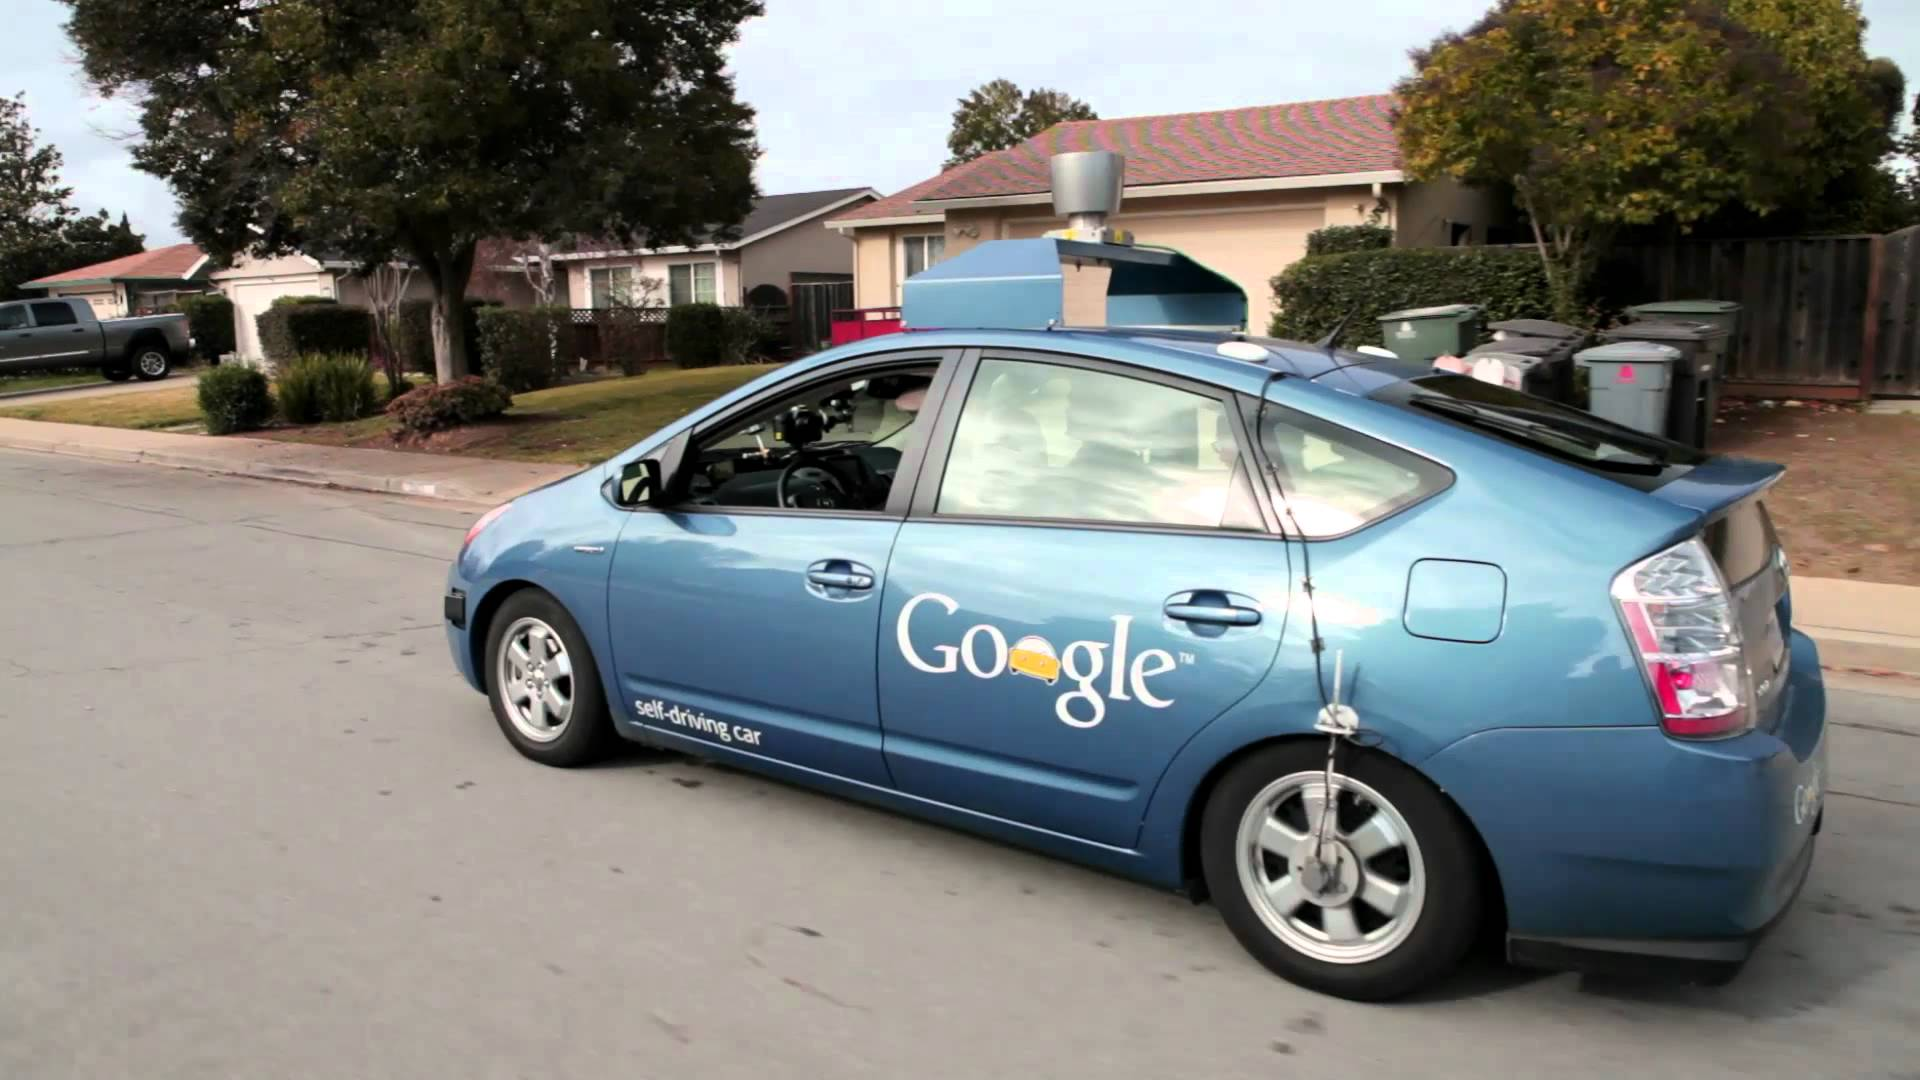
\includegraphics[width=\columnwidth]{img/google_vehicle.jpg}
	\caption[Google Self Driving Car]{An image of one of Google's self driving cars.}
	\label{fig:google_vehicle}
\end{figure}

Figure \ref{fig:google_vehicle} shows one of Google's fully autonomous vehicles.
To note is the LIDAR\footnote{LIDAR: LIght raDAR system.} sensor on the roof and the odometer visible on the back wheel.
Google has a fleet of vehicles – a dozen on the road at any given time – and has driven almost 500,000 kilometers with them in total \cite{www:google_blog_miles}.

\begin{figure}
	\centering
	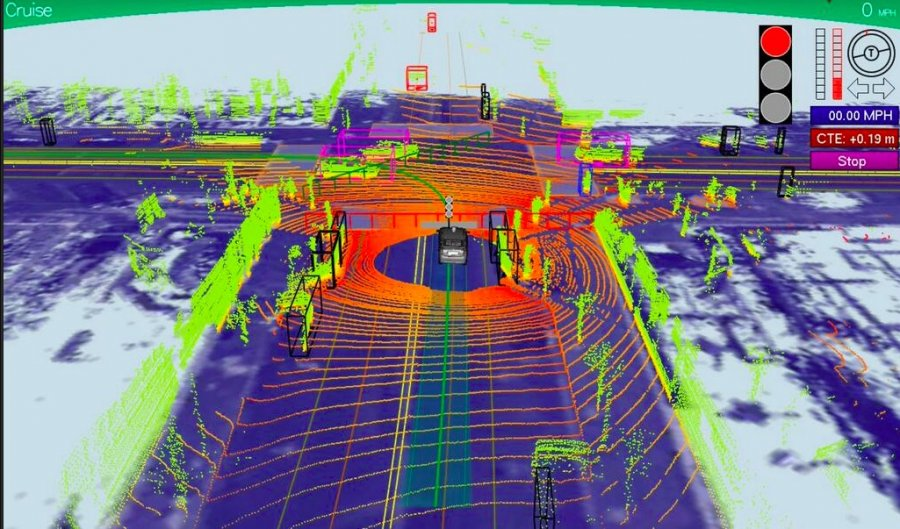
\includegraphics[width=\columnwidth]{img/google_tech_view.jpg}
	\caption[Tech View]{A screenshot of the digital representation shown to the vehicles' occupants for debugging purposes. This is a live view of the field of view of all the sensors of the vehicle rendered from a point of view behind and above the vehicle.}
	\label{fig:google_tech_view}
\end{figure}

The vehicle takes in its surroundings with a range of sensors and creates a digital representation of its surroundings.
This representation includes information of pedestrians and other vehicles, moving obstacles, the surroundings, information on the road, and the course that the vehicle plans on taking.
This digital representation is also available for the developers in the vehicle via a large screen that renders it, updating in real-time as the vehicle drives.
While primarily meant for debugging purposes, one journalist noted that such a view would alone already be nice to have in any modern vehicle, as there are no blind spots and it gives a nice overview of the road situation.
Figure \ref{fig:google_tech_view} shows a screenshot of the display.

Google's self driving car is currently only capable of driving under almost ideal situations.
If the car encounters a construction cite for example, it gives an auditory warning that the driver will have to take over control within the next mile, for example \cite{www:newyorker_google_car}.
The above citation is the only mention we found of how Google's vehicles handle the hand off.
Of course, given advanced warning only works if the vehicle has a chance of detecting the imminent hand off early enough to give the driver ample time to adjust and take over control from the automation.
Ideally of course, the vehicle would never have to hand control to its driver – but the technology is still a good bit away from that level of intelligence.
One must always keep in mind that computers have difficulties handling a task in an open system, such as driving a vehicle through a highly variable environment.

Google is not the only company working on developing self driving cars.
Mercedes-Benz also has a prototype in the works which has already successfully driven some distance \cite{www:mercedes_autonomous}.
From the video it is however clear that the car navigates on a predefined and mapped route that has been prepared for it.
To our knowledge, Google's cars do not require prepared courses.
However unlike Google, the vehicle uses only standard sensors commonly available – the LIDAR system is currently still relatively expensive and thus unsuited for mass production.
We have no knowledge on how the vehicle from Mercedes-Benz handles hand off.

\section{Control Interaction Issues}

This section explains interactions for controlling autonomous vehicles that already exist and issues that might and or will arise.
Most of the following content is however not based on hard research; consider it a proposal and extrapolation from available information without research backing it.

\subsection{General Assumptions}

Here we will briefly highlight what assumptions we make concerning autonomous vehicles.
One assumption we make is that the system will never actively cause an accident (due to fail-safe behavior), as has already been implemented in many robotic systems.
This is technically feasible and to our knowledge already implemented in the autonomous vehicles on the road today.
Note that a car rear-ending an autonomous vehicle is a passive accident, as the autonomous vehicle had no role in causing it.

The time frame in which hand off issues exist is also presumed to be constrained.
It will begin with the first autonomous vehicles, possibly before 2020, and end once all vehicles are autonomous and or networked together with a proven safety record.
Once such vehicles are the majority of vehicles on public roads, it seems logical to transfer control from the driver to a networked intelligence that is always in full control, as that allows the system to bypass the problem of human error.
Such advanced systems that can be fully trusted are however still many years away.
Even should a first world country have a fully autonomous vehicle network, less developed countries might not, meaning that automation might not work there because of a lack of required infrastructure.
Ideally of course the perfect autonomous vehicle would be fully capable of handling all situations safely by itself without driver interaction, but be capable of networking with other vehicles when required or when available to increase safety and efficiency.

\subsection{Vehicle Automation Interaction}

To better understand hand off issues, one must understand the basic interaction between machine and controller – in this case, vehicle and driver.
On the subject of sharing and trading control between automation and operator a subset of work exists which is relevant to the hand off issue for autonomous driving.

A general approach to the issue of sharing and trading control is to be found in the paper by Toshiyuki Inagaki \cite{inagaki:adaptive}.
In it, the author puts forth the notion that the sharing of control can be distinguished into three types: extension, relief, and partitioning.
Extension of control for example means that the computer simply assists the driver's task, of which power steering is a concrete example.
The second type, relief of control, is where most systems from section \ref{singular_systems} are located; they relieve some tasks from the driver, such as controlling vehicle speed.
Partitioning of control is then where the comprehensive systems as in section \ref{comprehensive_systems} are located.
The self driving car allows the driver to hand over the task of driving completely to the automation.
The driver's only remaining role would be to tell the vehicle where to drive to, effectively partitioning the task of traveling somewhere into two tasks that are divided between the automation and the driver.

For the topic of this paper, the third type of sharing control is the more important one.
The prototype self driving vehicles nowadays automatically execute actions, but allow the driver to veto all decisions by taking over control – which means that the driver actively steers and controls acceleration.
On the level of automation proposed by Sheridan and Verplanck \cite{sheridan:human}, such automation is on the sixth level out of ten, where the first level means that the human has full control and the tenth that the automation is fully in control.

However we must consider what happens when the vehicle, likely due to safety concerns, cannot decide on an automatic course of action in the case that it might endanger the life of its occupants.
This might be the case when an autonomous vehicle comes upon unknown road conditions – such as a section of road work – or when the vehicle suddenly cannot sense its surroundings – for example when a road has been snowed over.
The first example is easy to counter, due to the high probability that the vehicle can warn the driver well in advance that he will be required to take over control, possibly even long before the driver becomes aware of the obstruction.
The Google self driving car already does this; when it senses an upcoming construction site, it will warn the driver via auditory alarms and a notification on a display on the dashboard, compelling the driver to take over manual control \cite{www:newyorker_google_car}.

The more difficult situation is then the second example – mainly because it is time critical and involves handing over control when the driver might not have the required situational awareness.
Currently, self driving cars immediately fall down to the first level of automation, leaving all control to the driver.
For now this approach is sufficient, due to the nature of the projects and the careful use of the automation by people fully aware of the problems – mainly the engineers developing the systems.
Once self driving cars become publicly available, drivers will quickly come to trust the automation beyond what it is capable of doing due to a lack of understanding.
This is not a fault of the drivers – automation is meant to relieve humans of tasks – but a problem that requires a user friendly solution that can be readily implemented.

Beyond technical hurdles, psychological and driver experience issues must also be considered.
At some point in time after the mass introduction of autonomous vehicles, not being in direct control of the car at all times will become routine for most drivers, as such systems will have no trouble handling the majority of a drive by itself.
Even relatively easy tasks that the autonomous system can't handle might not be a problem when a driver has to intervene.
For the small percentage of critical situations however, implications of lacking experience could have large implications.
While autonomous cars already have a proven safety record, humans excel at handling situations where computers simply cannot function correctly, such as extraordinary situations for which the computer has no program to follow.
However human drivers require experience to correctly handle critical situations, or at least training that covers these situations.
If a vehicle can drive itself safely for the majority of a trip, driver skill will degrade over time.
This might well become a large problem in the future.
Overall, it is to assume that driving in general will become less accident-prone, but when critical situations do occur where driver interaction is required and time critical, errors that lead to accidents might actually increase.

Interaction issues will also become apparent in fringe cases where the driver is physically or mentally incapable of assuming control.
An example for this can be found in the promotional video by Google where a blind person is driven around by a self driving vehicle \cite{www:google_blind}.
Even the case of road construction where the car requires manual control becomes impossible to solve if the human can not or may not take control of the vehicle.
Also to be considered are situations where the car might realize that the driver is incapable of manually controlling the vehicle – be the driver drunk or too fatigued.
Even if they can safely move out of the way and await input from a qualified driver, this presents a significant usage hurdle for the technology.

Given such a possibility, it might even be generally better if the vehicle simply tries the best course of action it can, instead of trying to hand over control to a driver that might not be capable of offering any help to the situation at hand.
In that case the hand off becomes an even more serious risk, as the driver would then loose any chance of controlling the vehicle.
The question here is: can we allow the vehicle to forcibly retain control when the driver might make the situation worse?

We have now shown that the interaction between driver and autonomous vehicle in hand off situations can have serious implications for the utilization of autonomous vehicles.
While it seems likely that autonomous vehicles will function correctly and drive generally safer even today, the fringe cases where accidents can still happen should not be negated.

\subsection{Solutions}
\label{solutions}

Now that we have looked at the issue at hand, we will take a look at possible solutions, based off of existing systems and off domain work.
However we cannot, for previously stated reasons, offer up conclusively proven solutions.
For the most part the solutions are also not complete solutions to the problems at hand, but should decrease the risk of catastrophic failure in hand off situations at least.

A solution to the problem where the driver might not be capable or allowed to take manual control of the car lies in the levels of automation.
As stated previously, current autonomous vehicles drop to the first level of automation when human control is required.
This works from a technical viewpoint as long as the person is authorized to take direct control.
We propose an alternative system, where the computer would choose the level of control to drop down to depending on the circumstances.

To better visualize the proposal, we will explain it based on the example of a construction zone that the self driving car deems beyond its capabilities.
Instead of simply alerting the driver that manual control will be required to continue, the computer controlling the car might instead offer up alternative routes that take it around the obstacle.
The person in control of the car could then either allow the vehicle to pick the best alternative route or give it another destination.
By simply disallowing the car to traverse into a situation that would make manual control mandatory, the vehicle can remain in direct control and make manual override by the driver unnecessary.
In essence, we propose that if required or preferred, autonomous vehicles wouldn't drop to the first level of automation.
Instead, it would simply switch one down to the fifth level of automation, where the vehicle makes suggestions based on the information at hand, lets the human choose one, and then continues automatically by executing the selected one.
If the vehicle can network with others, another way around the issue would be to allow the autonomous vehicle to slave itself to a manual controlled car for the duration of the unknown situation.
This might actually be preferable in construction zones where pilot cars are utilized to allow vehicles to traverse the zone; self driving cars might simply create a chain of control.
Of course, the vehicle must still be aware of its surroundings and actively try to avoid collisions to the best of its abilities – it shouldn't trust the master vehicle fully.
That might mean that the chain of control is broken, in which case the car would effectively become stuck.

If the above solution is utilized to allow people to control a car without a license, it would allow them to interact with the vehicle in an abstracted way that would avoid giving them manual control.
It should work for the most cases where a not time critical hand off is required, meaning where enough time is available that the car can avoid the situation under its own control.
However for critical situations, the speed at which the vehicle can inform the occupants of a situation and receive instructions on how to avoid it becomes a significant bottleneck.
The car might not even be able to offer any solutions, effectively rendering this solution inadequate.
At that point, it might be of more use to use the vehicles' sensors to prepare the car for an imminent collision, for example by preparing seat-belts, airbags, and warning lights.

Another approach to the interaction issue comes from the driver side.
If the drivers remain capable of taking over control within the required time span, the problem can be decreased.
However, this requires two things: one, the driver is capable of handling the situation, and two, the driver can take over manual control quickly enough.

The first point is a matter of training and or experience.
As stated before, it is probable that without any outside motivation, driver experience will rapidly decrease for drivers controlling autonomous vehicles.
There is a range of options to prevent that from happening, or at the least to decrease the negative effects.
One option might be adapting the content and nature of attaining a driver's license.
Apart from learning the manual control of the vehicle, lessons might be mandatory for readying a driver to react correctly and fast enough in critical hand off situations.
This might include a range of situations, either simulated or on a prepared test course.
To make such special training effective, it should be required to test for, and if necessary, repeat it to allow drivers to keep their license active.
This would go hand in hand with the current trend of making driver's licenses limited for a specific time span, forcing drivers to continually prove that they are capable of safely controlling a vehicle.
Apart from forcing drivers to continuously remain trained, a better approach might be a more practical one: require drivers to drive a certain amount of their distance manually.
In the beginning, this might actually work nicely with gradually introducing autonomous vehicles to the general population.
It might be practical, for example, to allow autonomous control only on highways first.
This would serve four points rather nicely: one, highways are better suited as controlled environments, with a decreased risk of critical situations where the computer could not react better than a human driver.
Two, a significant percentage of people are loath to hand control of their vehicle to a computer \cite{www:power_study} – except for long voyages or instances where not the act of driving is the primary goal, but reaching the destination is.
Third, it would allow drivers to acquire and retain experience, as they would still be in manual control whenever driving on rural roads (with the added benefit that drivers could relax on long voyages and be better suited to driving when leaving the highway).
And fourth, the on and off ramps of highways can easily be used as controlled and viable hand off zones, without endangering other traffic.

The second problem, making sure that the driver is alert and always ready to take over, is a matter of feedback and alerts.
This is where the attention assist system could come into play.
By reading readily available sensor information from inside the vehicle – movement, volume, and gaze tracking – the vehicle can be aware of how aware the driver is.
This information can be used to enable the car to alert the driver when the computer determines him unfit to continue the voyage, offering to stop for a rest for example.
Such a system, if correctly implemented, should allow the vehicle to enforce alertness by the driver.
To supplement any passive sensors, one could also implement a dead man's switch as an active sensor.
This could be touch detection on the steering wheel or a switch the driver has to press in random intervals.

But even should the driver be alert and readily able to take over manual control, he might not immediately recognize a critical situation where the computer cannot remain in full control.
Such a situation might be ice rain, which might suddenly decrease the efficiency of the sensors used to drive enough that the computer cannot safely predict a path, while the driver could easily continue following the road.
Therefore, a good system for alerting the driver to take over must be in place.
To secure that the alarm reached the driver, we propose that such a system include not only visual, but also auditory and haptic feedback mechanism.
Visually, a prominent warning light within the vehicle should serve its purpose; accompany that with a warning alarm while the car also silences any entertainment systems should secure the undivided attention of the driver.
Add to that haptic feedback, for example rumbling the steering wheel or softly shaking the seat, and we have a system that uses three of the five senses of humans to alert the driver.

Even when the hand off is successful (implying that the driver is in full control of the vehicle and aware of the fact), he will take a moment to understand the situation – moments he might not have.
Even alerted the driver might lack information to behave correctly in a critical situation and be unable to process it quickly enough even if he has it.
To counter this, we propose making the overview view of what the car senses as seen for example in figure \ref{fig:google_tech_view} standard within all autonomous vehicles.
By reducing visual clutter, such a display should give an excellent overview of the cars surroundings, including the blind spots that drivers usually cannot perceive.
It should even be able to implement a system that highlights the problem the car encountered, allowing the driver to correctly assess the situation with a glance.
Beyond that, a heads-up-display that can display warnings and alerts on the windshield could also be of significant help.
Of course, any display would have to offer up a filtered view that is best suited to the capabilities of the driver.

Always remaining ready is however not a task that many humans can easily do – however they will still have a need of transportation for the foreseeable future.
To solve this, we propose a system for labeling automation systems in respect to driver capabilities.
Fully autonomous vehicles that would always drive so that no driver interaction is required would be free to use for everyone.
These might however be limited in where they drive and how fast they drive.
This would serve to allow the automation to drive in a safe environment that has the least amount of distractions possible, effectively rendering the need for a manual override to zero.
On the other side of the spectrum would be cars that can act fully autonomous when the computers deem it safe, but allow or even require the driver to take over when the situation warrants it.
These would only be available to drivers that have been certified for the safe operation of a fully autonomous vehicle.
This might be required when crossing into a new country where the laws governing driving are substantially different, rendering the automation incapable of functioning safely.

\section{Future Research}

Here we will offer a future outlook and where further work should and can be done.
These proposals are mainly based on the previous section, which offer up a range of questions and uncertainties that we will now highlight and use to suggest further work.

One topic that is worthy of research is how to warn the driver in critical hand off situations that he now has control – via auditory, visual, and or haptic feedback mechanisms.
Finding the right stimuli that alert the driver to the situation without distracting him from it will require studies and further work, with strong links to the psychological aspects of human information processing.
Such research might prove to be of the more immediate importance once fully autonomous vehicles become widely available.
Parallels could also be found in already existing systems from off domain fields, such as trains and airplanes.

Another interesting question is how to present the information the car continually gathers of its surroundings to the driver.
Again, making sufficient information available fast enough and easy to understand is not a trivial task.
One could consider for example that utilizing some artificial intelligence algorithms, the autonomous vehicle might decide by itself what range of information to present a driver and how to best present it.
This might lend itself to the topic because it allows the system to react adaptively to the needs and capabilities of the intended recipient – the driver.

To enable sound research, the autonomous vehicle field currently lacks a shared, public pool of raw data.
Therefore we would like to encourage companies and universities that have such data to make it publicly available, as it is essential for the safe development of interoperable self driving cars.
As in other domains where automation has been introduced, standards must be found that are strictly adhered to, based on common ground.

Apart form technical points or research that directly applies to the vehicles, more work can also be done for preparing and understanding human drivers in control of autonomous vehicles.
Studies into how to best prepare drivers for hand off situations under critical situations might be of further interest.

\section{Conclusion}

In this paper we have given an overview of the current state of automation technology in the automotive domain and off domain.
Based on this information, we have highlighted the problem of human-automation interaction for automotive applications.
Furthermore we have offered up points where solutions might be viable and formulated some concrete examples, although we lack any proof that they could be viable.
Therefore we have proposed some areas that could use some serious research work if non yet exists.

%{\small
% do not change the bibliography style
\bibliographystyle{abbrv}
\bibliography{sources}  
%}

\balancecolumns

\end{document}
